\section{基于Q学习的行为决策机制}
\subsection{Q表初始化}
实现Q-学习最简易的途径为通过Q表,该表格存储所有状态下采取各种动作后的奖励值,因而Q表的大小受限于状态和动作空间的数目。

在仿真平台中,基于强化学习控制的机器鼠(学习鼠)在产生行为时与规则鼠一样需要调用其动作执行层的接口函数,因此其动作空间为相应接口集合的子集。考虑到不同动作对行为交互的影响\cite{BarnettSTheRat},为降低Q表的大小,训练的复杂度,本文将前进、后退、左转、右转、梳理、被梳理、攀爬、匍匐共8种动作作为Q学习中的动作集合。

\begin{figure}[htbp]
  %\vspace{13pt}
  \centering
  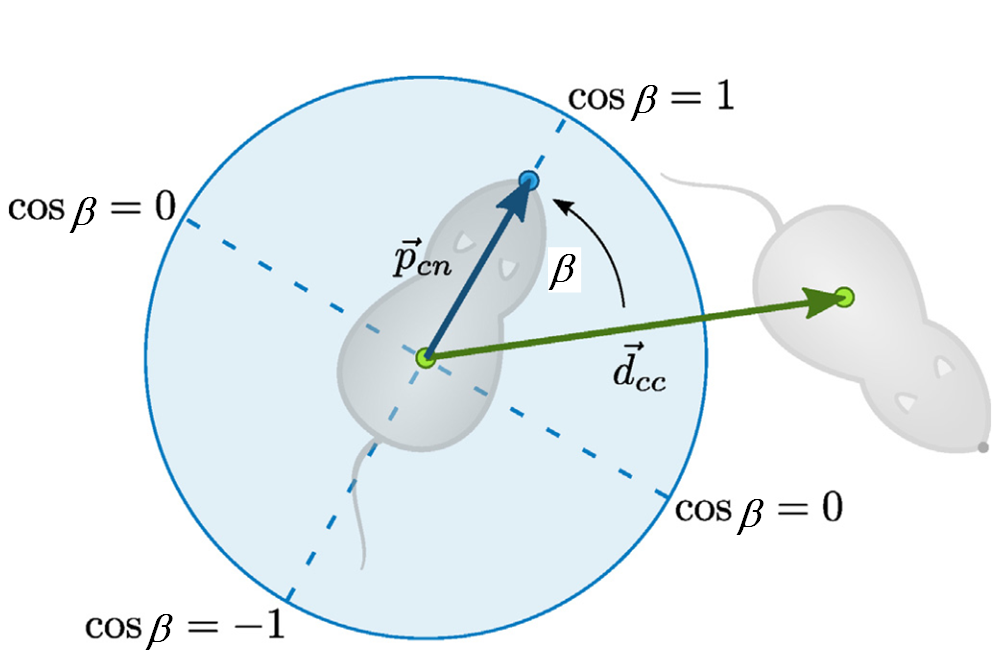
\includegraphics[width=0.4\linewidth]{images/ch04/relpose1.png}
  \caption{状态分类依据\cite{ISI:000436213800018}}\label{figure_relpos}
\end{figure}
对行为交互中过程的分类应当充分考虑生物鼠的行为决策依据。如图\ref{figure_relpos},\citeauthor{ISI:000436213800018}在研究生物鼠交互行为时利用相互间的相对位置确定所处状态,图中,$d_{cc}$表示两者中心点的距离,$\beta$为自身中心点与鼻端连线和自身中心点与交互对象中心点连线构成的夹角,考虑到角度具有对称性,用$\cos\beta$和$\sin\beta$的值进行划分\cite{ISI:000436213800018}。

同时考虑交互对象执行的动作对状态的影响,在两者距离较近时用动作进行状态分类。由此得到的行为交互中的状态共有背后、左侧、右侧、远距、梳理、被梳理、攀爬、匍匐、其他共9种。
% 各状态的量化指标为表\ref{tab:states}。
% \begin{table}[htbp]
%   \linespread{1.5}
%   \zihao{5}
%   \centering
%   \setlength{\fboxsep}{0cm}
%   \caption{学习鼠状态设置}\label{tab:states}
%   \begin{tabular}{m{2.5cm}<{\centering\arraybackslash}m{7.0cm}<{\centering\arraybackslash}m{2.0cm}<{\centering\arraybackslash}}
%     \toprule
%     状态 &  量化标准  & 图示\\ \midrule
%     $s_1$:背后         & $\sin\beta\leq-0.7.$ &\fbox{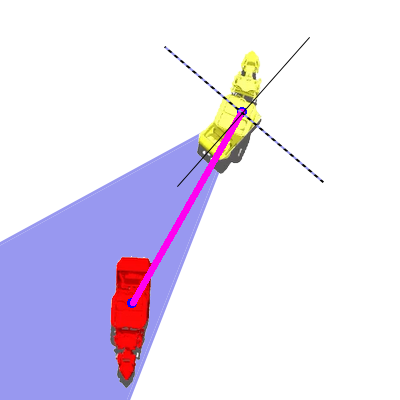
\includegraphics[height=1.7cm]{images/ch04/states/sback.png}}\\
%     $s_2$:左侧         & $-0.7<\sin\beta\leq0.7,\linebreak[1]\cos\beta<0.$ &\fbox{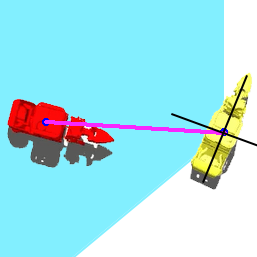
\includegraphics[height=1.7cm]{images/ch04/states/sleft.png}}\\
%     $s_3$:右侧         & $-0.7<\sin\beta\leq0.7,\linebreak[1]\cos\beta>0.$ &\fbox{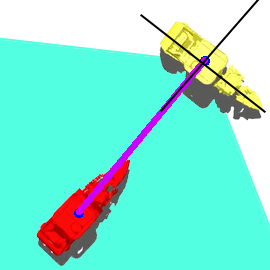
\includegraphics[height=1.7cm]{images/ch04/states/sright.png}}\\
%     $s_4$:远距         & $\sin\beta>0.7,{d}_{cc}\geq0.3~m.$ &\fbox{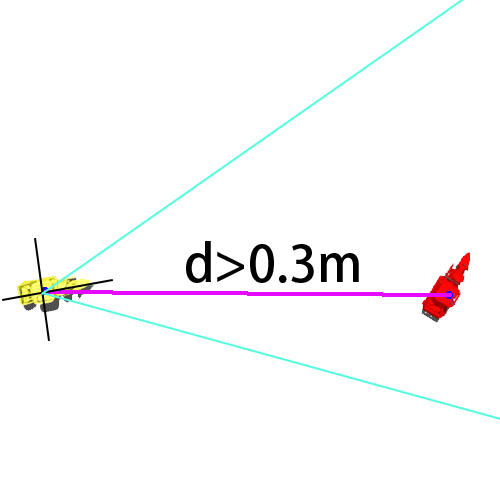
\includegraphics[height=1.7cm]{images/ch04/states/sfar.png}}\\
%     $s_5$:梳理         & $\sin\beta>0.7,{d}_{cc}<0.3~m$,\linebreak[2]交互对象动作为“梳理”。 &\fbox{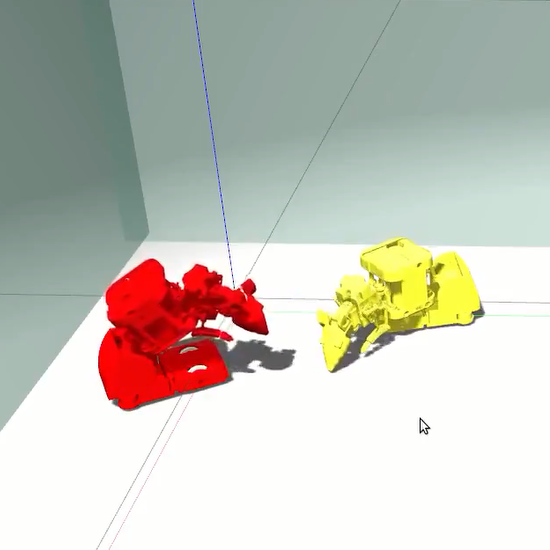
\includegraphics[height=1.7cm]{images/ch04/states/sgroom.png}}\\
%     $s_6$:被梳理     & $\sin\beta>0.7,{d}_{cc}<0.3~m$,\linebreak[2]交互对象动作为“被梳理”。  &\fbox{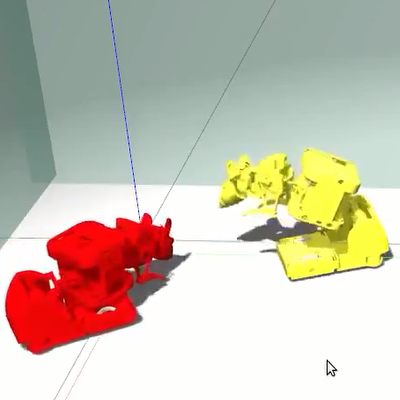
\includegraphics[height=1.7cm]{images/ch04/states/ssubgroom.png}}\\
%     $s_7$:攀爬        & $\sin\beta>0.7,{d}_{cc}<0.3~m$,\linebreak[2]交互对象动作为“攀爬”。  &\fbox{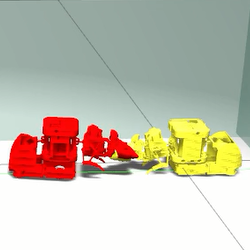
\includegraphics[height=1.7cm]{images/ch04/states/sup.png}}\\
%     $s_8$:匍匐         & $\sin\beta>0.7,{d}_{cc}<0.3~m$,\linebreak[2]交互对象动作为“匍匐”。  &\fbox{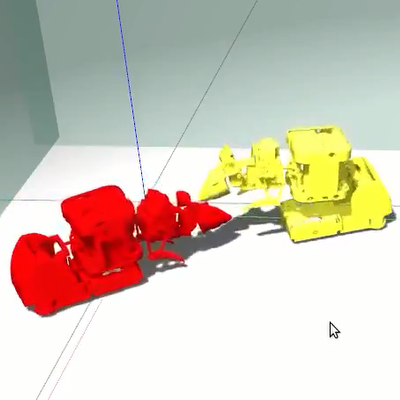
\includegraphics[height=1.7cm]{images/ch04/states/sunder.png}}\\
%     $s_9$:其他         & 上述状态以外的其他情况。 &$\times$\\
%     \bottomrule
%     \end{tabular}
% \end{table}

据此建立的Q表大小为$9\times8$,在程序中用二维数组表示。根据Q-学习算法(算法\ref{alg:Q-Learning}),Q表初始值可以是任意的,需要保证最终状态下所有动作的Q值为0($Q\left(terminal-state, ·\right)=0$)\cite{ISI:000481873900002},据此,本文将Q表中所有值均初始化为0。
\subsection{动作选择策略}
常见的Q-学习动作选择策略包括$\epsilon-$贪心算法($\epsilon-greedy$)、置信区间上界算法($UCB$)、汤普森采样($Thompson~sampling$)等,$\epsilon-greedy$算法实现较为简单,在各种情况下均有较好的适应性,能够较好地平衡“探索”和“利用”行为,因此本文选定其作为学习鼠的动作选择策略。

$\epsilon-greedy$算法的数学表达为式\ref{eq:epsilon-greedy},式中,$\pi\left(a^{*}|s\right)$表示学习鼠在状态$s$条件下做出动作$a^{*}$的概率,$\epsilon$为贪心率,取值范围为$[0,1]$,$m$为动作空间的大小。
\begin{equation}\label{eq:epsilon-greedy}
  \pi\left(a^{*}|s\right)=\begin{cases}
                        \displaystyle\frac{\epsilon}{m}+1-\epsilon, & \mbox{当 $a^{*}=arg\max\limits_{a\in \mathbb{A}}Q(s,a)$}  \\
                        \displaystyle\frac{\epsilon}{m}, & \mbox{其他}.
                      \end{cases}
\end{equation}

% 式\ref{eq:epsilon-greedy}表明,$\epsilon-greedy$算法具有以下四个特征:
% \begin{enumerate}[leftmargin=0em, listparindent=2em, parsep=0em, topsep=0em, label=(\theenumi)]
% %\setlength{\leftmargin}{0em}
% \setlength{\itemindent}{4em}
% \setlength{\labelsep}{0em}
% \setlength{\labelwidth}{2em}
% \setlength{\parsep}{0em}
% \setlength{\itemsep}{0em}
% \setlength{\topsep}{0em}
% %\setlength{\listparindent}{2em}
%   \item 能够保证持续的“探索”。
%   \item 动作集中的$m$个动作被执行的概率均不为0。
%   \item 有$1-\epsilon$的概率选择Q表中值最大的动作执行。
%   \item 有$\epsilon$的概率随机选择动作执行。
% \end{enumerate}

% 学习鼠的动作选择将按照算法\ref{alg:e-greddy-policy}实现。
% \begin{algorithm}[htb]
%   \caption{学习鼠动作选择策略}
%   \label{alg:e-greddy-policy}
%   \begin{algorithmic}[1]
%     \Require 当前状态$s$
%     \Ensure 应执行动作$a$
%     \State 在$[0,1]$中生成随机浮点数$r_{1}$;
%     \If{$r_{1}>\epsilon$}
%         \State 在$Q(s,·)$中寻找最大值索引$a^{*}$;
%         \State $a\gets a^{*}$;
%     \Else
%         \State 在$[1,m]$中生成随机整数$r_{2}$;
%         \State $a\gets \mathbb{A}(r_{2})$;
%     \EndIf
%     \State \Return a;
%   \end{algorithmic}
% \end{algorithm}

% $\epsilon-greedy$算法中,贪心率$\epsilon$决定着学习鼠进行“探索”的倾向。$\epsilon$值接近1时,学习鼠的动作选择具有更大的灵活性,能更快地对未知动作进行探索,进而有可能更快速适应环境的变化。反之,$\epsilon$值接近0时,学习鼠选择动作时将更多依靠已学习的知识,系统具有更强的稳定性。

% 本文设定$\epsilon$值为0.2,同时将$m=8$代入式\ref{eq:epsilon-greedy},计算得各动作选择概率为式\ref{eq:epsilon-greedy-value}。该式表明系统以$82.5\%$的概率选择Q表中的最大值对应的动作,当存在多个最大值时,系统将在其中随机选择。
% \begin{equation}\label{eq:epsilon-greedy-value}
%   \pi\left(a^{*}|s\right)=\begin{cases}
%                         0.825, & \mbox{当 $a^{*}=arg\max\limits_{a\in \mathbb{A}}Q(s,a)$}  \\
%                         0.025, & \mbox{其他}.
%                       \end{cases}
% \end{equation}
% \subsection{训练与更新}
% 在行为交互实验过程中,学习鼠需要不断观测环境反馈的奖励并据此更新Q表。在强化学习系统中,奖励起着至关重要的作用。这是由于延时奖励(delayed reward)是强化学习最困难的问题之一,现有研究表明,让奖励在接近最优解时大幅增加,有助于强化学习系统迅速收敛至最优解\cite{NgPolicyInvariance1999}。

% 基于这一理论,本文将当前状态与友好交互状态的距离作为奖励设计的指标。实现方式为:对学习鼠的所有状态进行价值评价,与友好交互距离近的状态价值高,反之与友好交互距离远的状态价值低。在行为交互中,友好交互状态指交互双方做出征服与服从、梳理与被梳理动作的协调状态。因此,对各状态的价值评价如表\ref{tab:evluate}所示。
% \begin{table}[htbp]
%   \linespread{1.5}
%   \zihao{5}
%   \centering
%   \caption{学习鼠状态价值评价}\label{tab:evluate}
%   \begin{tabular}{m{2cm}<{\centering\arraybackslash}*{9}{>{\centering\arraybackslash}m{0.8cm}}}
%     \toprule
%     状态$s$ & $s_1$ & $s_2$ & $s_3$ & $s_4$ & $s_5$ & $s_6$ & $s_7$ & $s_8$ & $s_9$ \\ \midrule
%     价值$V(s)$ & 0 & 2 & 2 & 3 & 10 & 10 & 8 & 8 & 6 \\
%     \bottomrule
%     \end{tabular}
% \end{table}

% 表\ref{tab:evluate}将行为交互中梳理与被梳理行为评价为最高,这是由于与攀爬和匍匐表现出的征服和服从相比,其攻击性更弱。而交互对象处于身后或较远处时的评价较低,是由于在不可见或距离较远的情况下的动作交互性较弱。

% 相应的,当状态转移时,学习鼠获得的奖励将按照式\ref{eq:reward}计算,式中,$S$为当前状态,$S'$为执行动作$A$后的状态,其范围均为$s_{1}\sim s_{9}$,$offset$为偏置,其作用是保证$S'=S$时学习鼠获得的奖励仍然为负值,这将有助于部分解决学习鼠面临的局部最优困境,本文设定其值为0.5。
% \begin{equation}
%     \label{eq:reward}
%     R(s_t=S,s_{t+1}=S')=V(S')-V(S)-offset.
% \end{equation}

% 将表\ref{tab:evluate}中各状态价值代入式\ref{eq:reward},得到即时奖励矩阵为表\ref{tab:reward_martrix}。
% \begin{table}[htbp]
%   \linespread{1.5}
%   \zihao{5}
%   \centering
%   \caption{学习鼠即时奖励矩阵}\label{tab:reward_martrix}
%   \begin{tabular}{p{1.5cm}<{\centering\arraybackslash}|*{9}{>{\centering\arraybackslash}p{0.8cm}}}
%     \toprule
%     \diagbox[width=1.8cm, height=1.2\line]{$S$}{$S'$} & $s_1$ & $s_2$ & $s_3$ & $s_4$  & $s_5$ & $s_6$ & $s_7$ & $s_8$ & $s_9$ \\ \midrule
%     $s_1$ & -0.5 &  1.5 & 1.5  & 2.5 & 9.5 & 9.5 & 7.5 & 7.5 & 5.5 \\
%     $s_2$ & -2.5 & -0.5 & -0.5 & 0.5 & 7.5 & 7.5 & 5.5 & 5.5 & 3.5 \\
%     $s_3$ & -2.5 & -0.5 & -0.5 & 0.5 & 7.5 & 7.5 & 5.5 & 5.5 & 3.5 \\
%     $s_4$ & -3.5 & -1.5 & -1.5 & -0.5 & 6.5 & 6.5 & 4.5 & 4.5 & 2.5 \\
%     $s_5$ & -10.5 & -8.5 & -8.5 & -7.5 & -0.5 & -0.5 & -2.5 & -2.5 & -4.5 \\
%     $s_6$ & -10.5 & -8.5 & -8.5 & -7.5 & -0.5 & -0.5 & -2.5 & -2.5 & -4.5 \\
%     $s_7$ & -8.5 & -6.5 & -6.5 & -5.5 & 1.5 & 1.5 & -0.5 & -0.5 & -2.5 \\
%     $s_8$ & -8.5 & -6.5 & -6.5 & -5.5 & 1.5 & 1.5 & -0.5 & -0.5 & -2.5 \\
%     $s_9$ & -6.5 & -4.5 & -4.5 & -3.5 & 3.5 & 3.5 & 1.5 & 1.5 & -0.5 \\
%     \bottomrule
%     \end{tabular}
% \end{table}

% 学习鼠观测到即时奖励$R$和下一状态$S'$后,学习鼠将按照式\ref{eq:update_qtable}更新Q表。式中包含学习率$\alpha$和遗忘率$\gamma$两个超参数,其中$\alpha$代表Q表更新时该步学到的Q值所占比重,其接近1表明新发现的信息将更加重要;$\gamma$代表了未来奖励的重要性,其接近1则意味着系统更重视长远奖励。%本文设定$\alpha=0.8,\gamma=0.8$。
% \begin{equation}\label{eq:update_qtable}
%   Q(S, A)=Q(S, A)+\alpha\left[R+\gamma\max\limits_{a\in\mathbb{A}}Q(S', a)-Q(S, A)\right]
% \end{equation}

% 在强化学习系统中,某轮训练到达最终状态则意味着该次训练结束,应当开始新一轮训练,例如围棋训练中一一盘棋具决出胜负作为其最终状态。在机器鼠行为交互仿真实验中,“最终状态”为规则鼠与学习鼠表现为友好的交互状态。但行为交互与围棋博弈存在不同,即使达到最终状态也并不意味着行为交互的终止,据此设定的即时奖励考虑状态间转移的情况,能够保证交互实验的持续开展。

% 学习鼠的训练流程可以用图\ref{figure_qlpipeline}表示。
% \begin{figure}[htbp]
%   %\vspace{13pt}
%   \centering
%   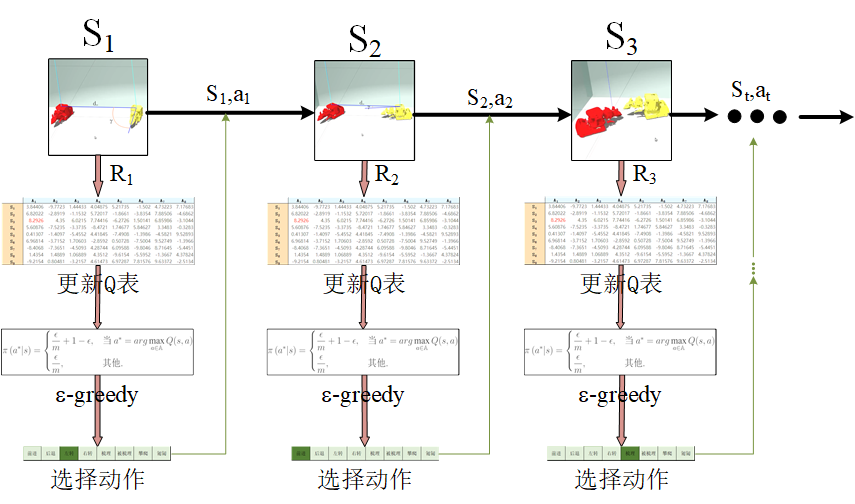
\includegraphics[width=0.95\linewidth]{images/ch04/pipeline.png}
%   \caption{学习鼠训练流程}\label{figure_qlpipeline}
% \end{figure} 